\begin{figure}[H]
\centering
\newcommand{\wmg}{0.34\columnwidth}  % width maunu growth
\newcommand{\hmg}{3.2cm}  % height maunu growth
\begin{tabular}{c}
\hspace{-0.3cm} \includegraphics[width=\wmg,height=\hmg]{\constructionfigsdir/decomposition/11-Feb-v4-03-mauna2003-s_max_level_0/03-mauna2003-s_all_small} 
\hspace{-0.3cm} \includegraphics[width=\wmg,height=\hmg]{\constructionfigsdir/decomposition/11-Feb-v4-03-mauna2003-s_max_level_1/03-mauna2003-s_all_small}
\hspace{-0.3cm} \includegraphics[width=\wmg,height=\hmg]{\constructionfigsdir/decomposition/11-Feb-v4-03-mauna2003-s_max_level_2/03-mauna2003-s_all_small}
\end{tabular}
\caption{Posterior mean and variance for different depths of kernel search.  The dashed line marks the extent of the dataset.  In the first column, the function is only modeled as a locally smooth function, and the extrapolation is poor.  Next, a periodic component is added, and the extrapolation improves.  At depth 3, the kernel can capture most of the relevant structure, and is able to extrapolate reasonably. %\TBD{RBG: (1) I think we somehow need to visualize the lengthscales, to make it obvious that the SE kernels really mean different things. (2) Why isn't SE + PE the correct answer?}
}
\label{fig:mauna_grow}
\end{figure}
